\documentclass[aspectratio=169]{beamer}
\usepackage{panqueques}
\title{Group and Surface}
\author{Ziang Wang}
\date{\today}
\usetikzlibrary{arrows}
\begin{document}

%title-page %%edit in 1-title-page folder
\begin{frame}[noframenumbering,plain]
    \begin{tikzpicture}[remember picture, overlay]
        \fill[black] (current page.south west) rectangle ([xshift=4cm]current page.north west);
        \node at ([xshift=2cm,yshift=-4.5cm]current page.north west) {
\includegraphics[width=3cm]{1-title-page/log.png}};
    \end{tikzpicture}
    \begingroup  
        \flushright
        {\fontfamily{qag}\selectfont\Huge\bfseries\color{black}\MyTitle}\vspace{1em}\\
        \MyAuthor\vspace{0.5em}\\
        \MyDate\par
    \endgroup
\end{frame}

%edit as needed

\begin{frame}[plain]
\centering \huge\color{black}\textbf{Fundamental Group of Surface}
\vspace{5mm}
$$\LARGE\textbf{Path} \Rightarrow \textbf{Loop} \Rightarrow \textbf{Surface}$$
\end{frame}
%%%%%%%%%%%%%%%%%%%%%%%%%%%%%%%%%%%%%%%%%%%%%%%%%%%%%%%%%%%%%%%%%%%%%%%%%%%%%%%%%%%%%%%%%%%%%%%%%%%%%%%%%%%%%%%%%%%%%%%%%%%%%%%%%%%%%%%%%%%%%%%%%%%%%%%%%%%%%%%%%%%%%%%%%%%%%%%%%%%%%%%%%%%%%%%%%%%
\begin{frame}{\textbf{Homotopy}}
    \begin{bee}[Path function]
        $$f: \quad [0,1] \mapsto X$$
    \end{bee}


\usetikzlibrary {arrows.meta}
\begin{figure}
   

\begin{tikzpicture}[scale=0.70]

\draw[-latex] (-0.8,1.5) -- (1.8,1.5) ; %edit here for the axis
\foreach \x in  {0,1} % edit here for the vertical lines
\draw[shift={(\x,1.5)},color=black] (0pt,3pt) -- (0pt,-3pt);
\foreach \x in {0,1} % edit here for the numbers
\draw[shift={(\x,1.5)},color=black] (0pt,0pt) -- (0pt,-3pt) node[below] 
{$\x$};
\draw[*-*] (-0.1,1.5) -- (1.1,1.5);
\draw[very thick] (-0.1,1.5) -- (1.1,1.5);

\draw[->] (3,1.5) -- (4,1.5);

% First, define nodes
\draw (6,0) node[circle, inner sep=0.8pt, fill=black, label={below:{$X_0$}}] (E) {};  
\draw (9,3) node[circle, inner sep=0.8pt, fill=black, label={below:{$X_1$}}] (F) {}; 

% Draw the curved line. No to[bend] is allowed, only explicit control points
\draw  (E) .. controls +(7.9,1) and +(4.1,1).. (F);
% Now, repeat the same curve, shifted up, and define 20 inner points named
% p1, p2, p3, etc.. for positions 0.15, 0.16, 0.17, etc up to 0.35 inside that curve
\path  ($(E)+(0,0.2)$) .. controls +(7.9,1) and +(4.1,1) ..  ($(F)+(0, 0.2)$)
 {\foreach \t [count=\i] in {0.15,0.16,...,0.35} {  coordinate[pos=\t] (p\i) } };

% Finally draw the "curve" (polygonal line indeed) through those 20 inner points
\draw[->>] (p1) { \foreach \i in {1,...,20} {-- (p\i) } };

\end{tikzpicture}
\caption{Path function}
    \label{fig:my_label}
\end{figure}

\end{frame}
%%%%%%%%%%%%%%%%%%%%%%%%%%%%%%%%%%%%%%%%%%%%%%%%%%%%%%%%%%%%%%%%%%%%%%%%%%%%%%%%%%%%%%%%%%%%%%%%%%%%%%%%%%%%%%%%%%%%%%%%%%%%%%%%%%%%%%%%%%%%%%%%%%%%%%%%%%%%%%%%%%%%%%%%%%%%%%%%%%%%%%%%%%%%%%%%%%%
\begin{frame}{\textbf{Homotopy}}
    \begin{bee}[Definition]
        $f$ and $f'$ are two continuous maps. If there is a continuous function $H$ that 
        $$H: \quad X \times [0,1] \rightarrow Y$$
        $$H(x,0)=f(x) \quad \textbf{and} \quad H(x,1)=f'(x)$$
        $f$ is then homotopic to $f'$, denoted as $f \simeq f'$
    \end{bee} 
\begin{figure}
    \centering
    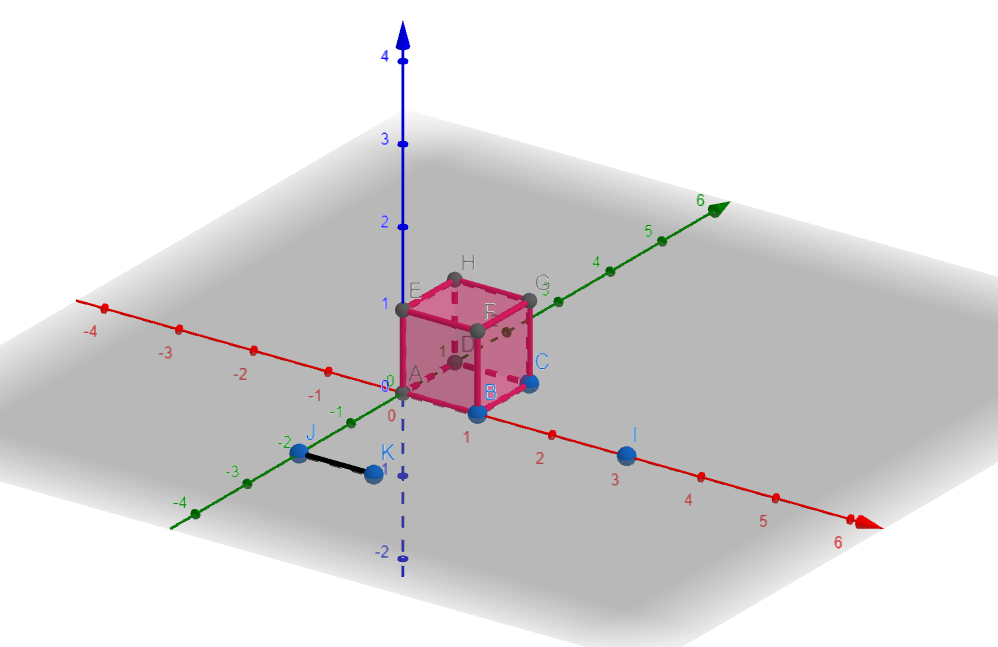
\includegraphics[scale=0.4]{1}
    \caption{Straight line homotopy}
    \label{fig:my_label}
\end{figure}
\end{frame}
%%%%%%%%%%%%%%%%%%%%%%%%%%%%%%%%%%%%%%%%%%%%%%%%%%%%%%%%%%%%%%%%%%%%%%%%%%%%%%%%%%%%%%%%%%%%%%%%%%%%%%%%%%%%%%%%%%%%%%%%%%%%%%%%%%%%%%%%%%%%%%%%%%%%%%%%%%%%%%%%%%%%%%%%%%%%%%%
\begin{frame}{\textbf{Homotopy}}
\begin{figure}
    \centering
   \begin{tikzpicture}[scale=0.9]

% First, define nodes
\draw (0,0) node[circle, inner sep=0.8pt, fill=black, label={below:{$E$}}] (E) {};  
\draw (5,0) node[circle, inner sep=0.8pt, fill=black, label={below:{$F$}}] (F) {}; 

% Draw the curved line. No to[bend] is allowed, only explicit control points
\draw  (E) .. controls +(1.9,1) and +(-1.9,1).. (F);
% Now, repeat the same curve, shifted up, and define 20 inner points named
% p1, p2, p3, etc.. for positions 0.15, 0.16, 0.17, etc up to 0.35 inside that curve
\path  ($(E)+(0,0.2)$) .. controls +(1.9,1) and +(-1.9,1) ..  ($(F)+(0, 0.2)$)
 {\foreach \t [count=\i] in {0.15,0.16,...,0.35} {  coordinate[pos=\t] (p\i) } };

% Finally draw the "curve" (polygonal line indeed) through those 20 inner points
\draw[->>] (p1) { \foreach \i in {1,...,20} {-- (p\i) } };

% A second example, with the same ideas but different path
\draw[red]  (E) .. controls +(2,-2) and +(-3,-1).. (F);
\path  ($(E)+(0,0.2)$) .. controls +(2,-2) and +(-3,-1)..  ($(F)+(0, 0.2)$) 
{\foreach \t [count=\i] in {0.15,0.16,...,0.55} {  coordinate[pos=\t] (p\i) } };

\draw[red, ->>] (p1) { \foreach \i in {1,...,40} {-- (p\i) } };

%third
\draw[blue]  (E) .. controls +(2.4,1.9) and +(-2.7,-2).. (F);
\path  ($(E)+(0,0.2)$) .. controls +(2.4,1.9) and +(-2.7,-2)..  ($(F)+(0, 0.2)$) 
{\foreach \t [count=\i] in {0.15,0.16,...,0.55} {  coordinate[pos=\t] (p\i) } };

\draw[blue, ->>] (p1) { \foreach \i in {1,...,40} {-- (p\i) } };

\end{tikzpicture}
    \caption{Homotopy equivalent class}
    \label{fig:my_label}
\end{figure}
\begin{bee}[] 
      Equivalence class: $[f]$
\end{bee} 
\end{frame}
%%%%%%%%%%%%%%%%%%%%%%%%%%%%%%%%%%%%%%%%%%%%%%%%%%%%%%%%%%%%%%%%%%%%%%%%%%%%%%%%%%%%%%%%%%%%%%%%%%%%%%%%%%%%%%%%%%%%%%%%%%%%%%%%%%%%%%%%%%%%%%%%%%%%%%%%%%%%%%%%%%%%%%%%%%%%%%%
\begin{frame}{\textbf{Group}} 
    \begin{bee}[Definition] 
        Group is a set $G$ with an operation $\ast$ that satisfies: \\
         \begin{enumerate}[$\bullet$]
            \item There exists an identity element $e \in G$. 
            \item If $\alpha \in G$, then its inverse $\alpha^{-1} \in G$.
            \item Associativity
        \end{enumerate} 
    \end{bee} 
e.g \\ 
\hspace{5mm}$\mathbf{N}$ is not a group under $+$, but $\mathbf{Z}$ is.
\end{frame}
%%%%%%%%%%%%%%%%%%%%%%%%%%%%%%%%%%%%%%%%%%%%%%%%%%%%%%%%%%%%%%%%%%%%%%%%%%%%%%%%%%%%%%%%%%%%%%%%%%%%%%%%%%%%%%%%%%%%%%%%%%%%%%%%%%%%%%%%%%%%%%%%%%%%%%%%%%%%%%%%%%%%%%%%%%%%%%%%%%%%%%%%%%%%%%%%%%%
\begin{frame}{Homotopy group}
\begin{bee}[] 
      Now we generate a free group using homotopy equivalence class under the operation $\ast$
      $$[a]\ast[b] = [a \ast b]$$
      $$G = \prod^{\ast}G_{\alpha}$$
      $$G_{\alpha} = \prod^{\ast}[a_\alpha] \quad \textbf{or}\quad G_{\alpha} \hspace{2mm}\supseteq\hspace{2mm} \{x \ast y \hspace{2mm} | \hspace{2mm}  x,y \in [\alpha_i] \}$$
\end{bee} 
\begin{figure}
   

\begin{tikzpicture}[scale=0.70]

% First, define nodes
\draw (0,0) node[circle, inner sep=0.8pt, fill=black, label={below:{$X_0$}}] (E) {};  
\draw (3,0) node[circle, inner sep=0.8pt, fill=black, label={below:{$X_1$}}] (F) {}; 
\draw (8,0) node[circle, inner sep=0.8pt, fill=black, label={below:{$X_2$}}] (H) {};

% Draw the curved line. No to[bend] is allowed, only explicit control points
\draw  (E) .. controls +(0.3,-1) and +(1,0).. (F);
% Now, repeat the same curve, shifted up, and define 20 inner points named
% p1, p2, p3, etc.. for positions 0.15, 0.16, 0.17, etc up to 0.35 inside that curve
\path  ($(E)+(0,0.2)$) .. controls +(0.3,-1) and +(1,0) ..  ($(F)+(0, 0.2)$)
 {\foreach \t [count=\i] in {0.15,0.16,...,0.35} {  coordinate[pos=\t] (p\i) } };

% Finally draw the "curve" (polygonal line indeed) through those 20 inner points
\draw[->>] (p1) { \foreach \i in {1,...,20} {-- (p\i) } };

% Draw the curved line. No to[bend] is allowed, only explicit control points
\draw  (F) .. controls +(3.1,1) and +(3.5,1).. (H);
% Now, repeat the same curve, shifted up, and define 20 inner points named
% p1, p2, p3, etc.. for positions 0.15, 0.16, 0.17, etc up to 0.35 inside that curve
\path  ($(F)+(0,0.2)$) .. controls +(3.1,1) and +(3.5,1) ..  ($(H)+(0, 0.2)$)
 {\foreach \t [count=\i] in {0.15,0.16,...,0.35} {  coordinate[pos=\t] (p\i) } };

% Finally draw the "curve" (polygonal line indeed) through those 20 inner points
\draw[->>] (p1) { \foreach \i in {1,...,20} {-- (p\i) } };
\end{tikzpicture}
\caption{$f \ast f'$}
    \label{fig:my_label}
\end{figure}
 
\end{frame}
%%%%%%%%%%%%%%%%%%%%%%%%%%%%%%%%%%%%%%%%%%%%%%%%%%%%%%%%%%%%%%%%%%%%%%%%%%%%%%%%%%%%%%%%%%%%%%%%%%%%%%%%%%%%%%%%%%%%%%%%%%%%%%%%%%%%%%%%%%%%%%%%%%%%%%%%%%%%%%%%%%%%%%%%%%%%%%%%%%%%%%%%%%%%%%%%%%%
\begin{frame}{Fundamental Group}
 \begin{bee}[] 
        The easiest homotopy group: \\
        $$\pi_1(X,x_0)$$
    \end{bee} 

\begin{figure}
\begin{tikzpicture}[scale= 0.9]

% First, define nodes
\draw (0,0) node[circle, inner sep=0.8pt, fill=black, label={below:{$X_0$}}] (E) {};  
\draw (0,0) node[circle, inner sep=0.8pt, fill=black, label={below:{}}] (F) {}; 


% Draw the curved line. No to[bend] is allowed, only explicit control points
\draw  (E) .. controls +(4,2) and +(-1,3).. (F);
% Now, repeat the same curve, shifted up, and define 20 inner points named
% p1, p2, p3, etc.. for positions 0.15, 0.16, 0.17, etc up to 0.35 inside that curve
\path  ($(E)-(-0.3,0)$) .. controls +(4,2) and +(-1,3) ..  ($(F)-(-0.3, 0)$)
 {\foreach \t [count=\i] in {0.15,0.16,...,0.35} {  coordinate[pos=\t] (p\i) } };

% Finally draw the "curve" (polygonal line indeed) through those 20 inner points
\draw[->>] (p1) { \foreach \i in {1,...,20} {-- (p\i) } };

\end{tikzpicture}
\caption{Fundamental Group}
    \label{fig:my_label}
\end{figure}


\end{frame}
%%%%%%%%%%%%%%%%%%%%%%%%%%%%%%%%%%%%%%%%%%%%%%%%%%%%%%%%%%%%%%%%%%%%%%%%%%%%%%%%%%%%%%%%%%%%%%%%%%%%%%%%%%%%%%%%%%%%%%%%%%%%%%%%%%%%%%%%%%%%%%%%%%%%%%%%%%%%%%%%%%%%%%%%%%%%%%%%%%%%%%%%%%%%%%%%%%%
\begin{frame}{Fundamental Group of Surface}
 \begin{bee}[Polygonal region scheme]
Assign each edge with a label. Default direction is set as from $p_{k-1}$ to $p_{k}$.\\
Labelling scheme:
$$w = (a_1)^{\epsilon_1} \ast       (a_2)^{\epsilon_2} \ast    (a_3)^{\epsilon_3} \ast (a_4)^{\epsilon_4} \ast...        \ast(a_n)^{\epsilon_n} $$
where $\epsilon = \pm 1$    
    \end{bee} 
Note: This is an element of the free group generated by homoptopic equivalence class!
\end{frame}
%%%%%%%%%%%%%%%%%%%%%%%%%%%%%%%%%%%%%%%%%%%%%%%%%%%%%%%%%%%%%%%%%%%%%%%%%%%%%%%%%%%%%%%%%%%%%%%%%%%%%%%%%%%%%%%%%%%%%%%%%%%%%%%%%%%%%%%%%%%%%%%%%%%%%%%%%%%%%%%%%%%%%%%%%%%%%%%%%%%%%%%%%%%%%%%%%%%
\begin{frame}{Fundamental Group of Surface}
 \begin{figure}
     \centering
     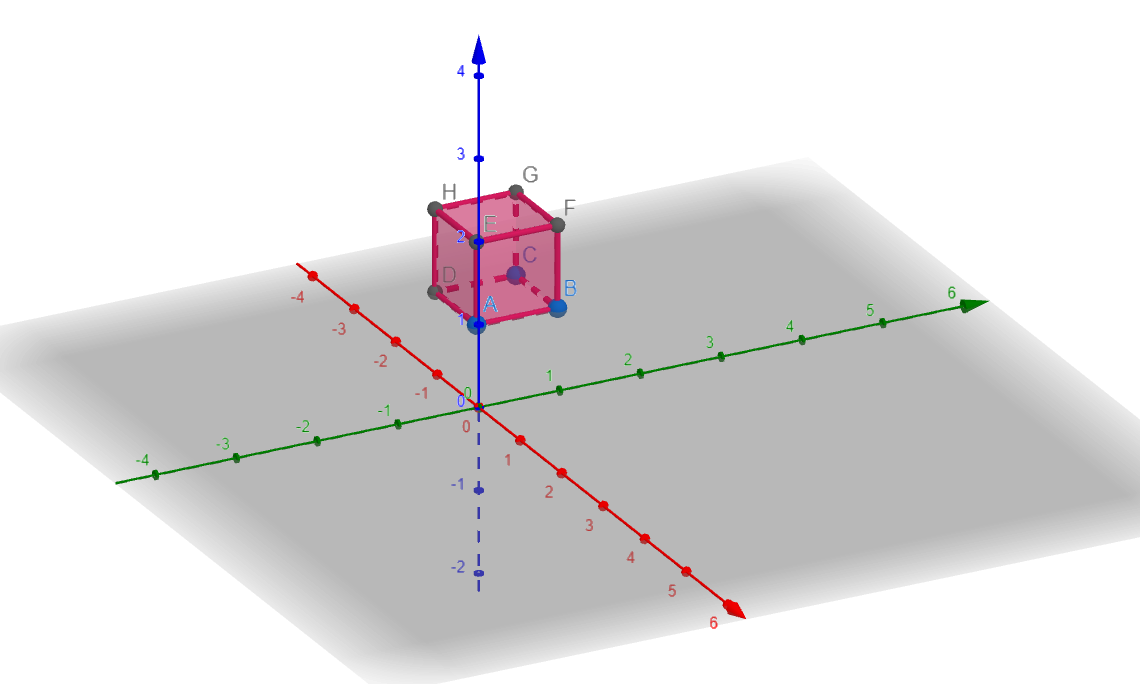
\includegraphics[scale=0.45]{2}
     \caption{torus}
     \label{fig:my_label}
 \end{figure}
$$w = a_1 \cdot b_{1}^{-1} \cdot a_{2}^{-1} \cdot b_2 \textbf{ and } a_1 \sim a_2, b_1 \sim b_2$$
\end{frame}
%%%%%%%%%%%%%%%%%%%%%%%%%%%%%%%%%%%%%%%%%%%%%%%%%%%%%%%%%%%%%%%%%%%%%%%%%%%%%%%%%%%%%%%%%%%%%%%%%%%%%%%%%%%%%%%%%%%%%%%%%%%%%%%%%%%%%%%%%%%%%%%%%%%%%%%%%%%%%%%%%%%%%%%%%%%%%%%%%%%%%%%%%%%%%%%%%%%
\begin{frame}{Fundamental Group of Surface}
 \begin{figure}
     \centering
     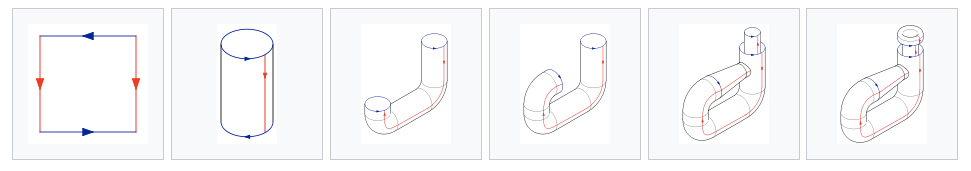
\includegraphics[scale=0.4]{3}
     \caption{Klein Bottle}
     \label{fig:my_label}
 \end{figure}
$$w = a_{1}^{-1} \cdot b_{1} \cdot a_{2}^{-1} \cdot b_2^{-1} \textbf{ and } a_1 \sim a_2, b_1 \sim b_2$$
\end{frame}





%reference %%edit in 3-reference folder
\begin{frame}{References}
    \nocite{apostol2004mathematical}
    \nocite{fraleigh2003first}
    \bibliographystyle{plain}
    \bibliography{3-reference/ref.bib}
\end{frame}

\end{document}